\documentclass[../main.tex]{subfiles}

\graphicspath{{../images/}}

\begin{document}
\pagestyle{fancy}
\lhead{Homework 4}
\chead{Junseo Shin}
\rhead{PHYS 421}

\setcounter{section}{4}

% 3.4, 3.7, 3.8, 3.10, 3.11, 3.13 
\paragraph{3.4} 
\begin{enumerate}
    \item [(a)] Average field over a spherical surface due to charges outside the sphere is the same at the center:

    For a charge $q$ a distance $z$ above the center of the sphere, 
    we can use the same geometrical argument from HW 2 Problem 2.7:
    The average field at over the surface will be in the negative $z$ direction
    \begin{align*}
        \vb E = \ke \frac{q}{\scriptr^2} \cos\psi (-\vu z)
    \end{align*}
    where (using law of cosines)
    \begin{align*}
        \scriptr^2 = z^2 + R^2 - 2zR\cos\theta \qquad \cos\phi = \frac{z - R\cos\theta}{\scriptr}
    \end{align*}
    The surface element is $\dd a = R^2 \sin\theta \dd \theta \dd\phi$, so the average field is 
    \begin{align*}
        \vb E_\text{avg} &= \frac{1}{4\pi R^2} \ke (-qR^2) \vu z \int_0^{2\pi} \int_0^\pi \frac{z - R\cos\theta}{(z^2 + R^2 - 2zR\cos\theta)^{3/2}} \sin \theta \dd\theta \dd\phi \\
        &= \frac{1}{4\pi} \ke (-q) \vu z (2\pi) \int_0^\pi \frac{z - R\cos\theta}{(z^2 + R^2 - 2zR\cos\theta)^{3/2}} \sin \theta \dd\theta \\
        &= \ke \frac{-q}{2} \vu z f
    \end{align*}
    The integral evaluates to (from Problem 2.7):
    Using the substitution $u = \cos\theta$: $\dd{u} = -\sin\theta \dd{\theta}$, and the limits of
    integration are $[\cos{0}, \cos{\pi}]$. So,
    \begin{align*}
        f(\theta) &= -\int_{1}^{-1} \frac{z - Ru}{(z^2 + R^2 - 2zRu)^{3/2}} \dd{u} \\
        &= \int_{-1}^{1} \frac{z - Ru}{(z^2 + R^2 - 2zRu)^{3/2}} \dd{u}
    \end{align*}
    substituting again with $v = \sqrt{z^2 + R^2 - 2zRu}$; $\dd{v} = \dfrac{zR}{v} \dd{u}$; and $
    u = \dfrac{1}{2zR}(z^2 + R^2 - v^2)$:
    \begin{align*}
        f(v) &= -\frac{1}{zR} \int \frac{z - \frac{1}{2z}(z^2 + R^2 - v^2)}{v^3} v \dd{v} \\
        &= -\frac{1}{2z^2R} \int \frac{2z^2 - (z^2 + R^2 - v^2)}{v^2} \dd{v} \\
        &= -\frac{1}{2z^2R} \int \frac{v^2 + z^2 - R^2}{v^2} \dd{v} \\
        &= -\frac{1}{2z^2R} \int \qt(1 + \frac{z^2 - R^2}{v^2}) \dd{v} \\
        &= -\frac{1}{2z^2R} \qt(v - \frac{z^2 - R^2}{v})
    \end{align*}
    substituting back in $v = \sqrt{z^2 + R^2 - 2zRu}$,
    \begin{align*}
        f(u) &= -\frac{1}{2z^2R} \qt(\frac{z^2 + R^2 - 2zRu}{\sqrt{z^2+R^2-2zRu}} 
            - \frac{z^2 - R^2}{\sqrt{z^2 + R^2 - 2zRu}}) \eval_{-1}^1 \\
        &= -\frac{1}{2z^2R} \qt(\frac{2R^2 - 2zRu}{\sqrt{z^2+R^2-2zRu}}) \eval_{-1}^1 \\
        &= \frac{1}{z^2} \qt(\frac{zu - R}{\sqrt{z^2+R^2-2zRu}}) \eval_{-1}^1 \\
        &= \frac{1}{z^2} \qt(
            \frac{z - R}{\sqrt{z^2 + R^2 - 2zR}} - \frac{-z - R}{\sqrt{z^2 + R^2 + 2zR}}
        ) \\
        &= \frac{1}{z^2}\qt(\frac{z - R}{\sqrt{z^2 + R^2 - 2zR}} + \frac{z + R}{z + R}) \\
        &= \frac{1}{z^2}\qt(\frac{z - R}{\sqrt{z^2 + R^2 - 2zR}} + 1)
    \end{align*}
    where the positive root $\sqrt{z^2 + R^2 - 2zR} = (z - R)$ for $z > R$, so
    \begin{align*}
        \vb E_\text{avg} = \ke \qt(-\frac{q}{2z^2}) \qt(\frac{z - R}{z - R} + \frac{z + R}{z + R}) \vu z
    \end{align*} 
    Simplfying to
    \begin{align*}
        \boxed{
            \vb E_\text{avg} = -\ke \frac{q}{z^2} \vu z
        }
    \end{align*}
    which is the same as the field at the center of the sphere.
    For a collection of particles, we can use superposition and find the net field as the sum of the fields at the center from each charge.
    \item [(b)] For charges inside the sphere we can use the result from before: for one charge
    \begin{align*}
        \vb E_\text{avg} = -\ke \frac{q}{z^2} \qt(\frac{z - R}{\sqrt{z^2 + R^2 - 2zR}} + \frac{z + R}{z + R}) \vu z
    \end{align*}
    but now the positive root is $\sqrt{z^2 + R^2 - 2zR} = (R - z)$ for $z < R$, so
    \begin{align*}
        \vb E_\text{avg} &= -\ke \frac{q}{z^2} \qt(\frac{z - R}{R - z} + \frac{z + R}{z + R}) \vu z \\
        &= -\ke \frac{q}{z^2} \qt(-1 + 1) \vu z \\
        \vb E_\text{avg} &= 0
    \end{align*}
    And we can superimpose the fields from a collection of charges 
    \begin{align*}
        \boxed{
            \vb E_\text{avg} = 0 + 0 + \cdots = 0
        }
    \end{align*}
\end{enumerate}

\newpage
\paragraph{3.7} Charges $+q$ \& $-2q$ are respectively $z = 3d$ \& $z = d$ above the $xy$ plane (grounded conductor). Find the force of the charge $+q$:

We can use the method of images and replace the grounded conductor with two charges $-q$ at $z = -3d$ and $+2q$ at $z = -d$. 
Thus the force on $+q$ is the superposition of the forces from the three charges:
The seperation vectors are 
\begin{align*}
    \vb \scriptr_{-2q} &= 2d \vu z \\
    \vb \scriptr_{+2q} &= 4d \vu z \\
    \vb \scriptr_{-q} &= 6d \vu z
\end{align*}
Finally, the force on charge $+q$ is
\begin{align*}
    \vb F &= \vb F_{-2q} + \vb F_{+2q} + \vb F_{-q} \\
    &= \ke \qt(
        \frac{-2q^2}{(2d)^2} + \frac{2q^2}{(4d)^2} + \frac{-q^2}{(6d)^2}
    ) \vu z \\
    &= \ke \frac{q^2}{d^2} \qt(-\frac{1}{2} + \frac{1}{8} - \frac{1}{36}) \vu z
\end{align*}
which simplifies to
\begin{align*}
    \boxed{
        \vb F = \ke \frac{29q^2}{72d^2} \vu z
    }
\end{align*}

\newpage
\paragraph{3.8} 
From Griffiths,
\begin{figure*}[ht]
    \centering
    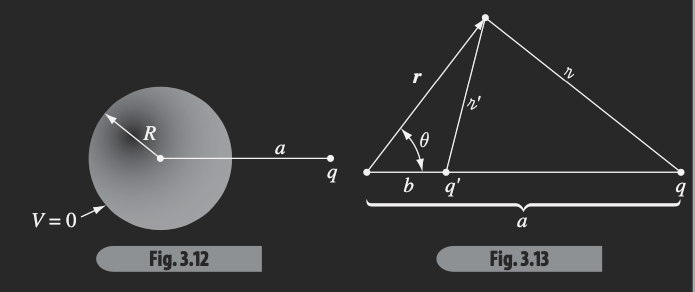
\includegraphics[width=0.5\linewidth]{hw3_8.png}
    \caption{From Griffiths Example 3.2}
    \label{fig:3.8}
\end{figure*}
where the configuration has another point charge
\begin{align*} \tag{3.15} \label{3.15}
    q' = -\frac{R}{a} q
\end{align*}
placed a distance
\[ \tag{3.16} \label{3.16} b = \frac{R^2}{a} \]
thus the potential of the config\begin{align*} \tag{3.17} \label{3.17}
    V (\vb r) = \ke \qt(
        \frac{q}{\scriptr} + \frac{q'}{\scriptr'}
    )
\end{align*}

\begin{itemize}
    \item [(a)] 
    Using law of cosines, show that Eq. \eqref{3.17} can be written as
    \begin{align*}
        V(r, \theta) = \ke \qt[
            \frac{q}{\sqrt{r^2 + a^2 - 2ra\cos\theta}} - \frac{q}{\sqrt{R^2 + (ra / R)^2 - 2ra \cos\theta}}
        ]
    \end{align*}

    From Fig. \ref{fig:3.8}, we can see that
    \begin{align*}
        \scriptr = \sqrt{r^2 + a^2 - 2ra \cos\theta} \qquad \scriptr' = \sqrt{r^2 + b^2 - 2rb \cos\theta}
    \end{align*}
    so using Eq. \eqref{3.15} and Eq. \eqref{3.16} we can rewrite
    \begin{align*}
        \frac{q'}{\scriptr'} &= \frac{-R}{a} \frac{q}{\sqrt{r^2 + (R^2 / a)^2 - 2r(R^2 / a) \cos\theta}} \\
        &= -\frac{1}{\sqrt{\frac{a^2}{R^2}}} \frac{q}{\sqrt{r^2 + (R^2 / a)^2 - 2r(R^2 / a) \cos\theta}} \\
        &= -\frac{q}{\sqrt{r^2 a / R^2 + (R^2 / a)^2 a^2 / R^2 - 2r(R^2 / a) \cos\theta} a^2 / R^2} \\
        \frac{q'}{\scriptr'} &= -\frac{q}{\sqrt{R^2 + (ra / R)^2 - 2ra \cos\theta}}
    \end{align*}
    Now we can rewrite Eq. \eqref{3.17} as
    \begin{align*}
        V = \ke \qt[
            \frac{q}{\sqrt{r^2 + a^2 - 2ra\cos\theta}} - \frac{q}{\sqrt{R^2 + (ra / R)^2 - 2ra \cos\theta}}
        ]
    \end{align*}
    \newpage
    \item [(b)] Finding the induced charge on the sphere \& integrating to get total induced charge:
    The normal component of the potential is $\vu n = \vu r$, so
    \begin{align*}
        \sigma &= -\epsilon_0 \pdv{V}{r} \eval_{r = R} \\
        &= -\epsilon_0 \ke q \qt(-\frac{1}{2}) \qt[
            \frac{2r - 2a\cos\theta}{(r^2 + a^2 - 2ra\cos\theta)^{3/2}}
            - \frac{2r a^2/R^2 - 2a \cos\theta}{(R^2 + (ra / R)^2 - 2ra \cos\theta)^{3/2}}
        ] \eval_{r = R} \\
        &= \frac{q}{4\pi} \qt[
            \frac{R - a\cos\theta}{(R^2 + a^2 - 2Ra\cos\theta)^{3/2}}
            - \frac{a^2 / R - a \cos\theta}{(R^2 + a^2 - 2Ra \cos\theta)^{3/2}}
        ] \\
        &= \frac{q}{4\pi} \qt[
            \frac{R - a^2 / R}{(R^2 + a^2 - 2Ra\cos\theta)^{3/2}}
        ]
    \end{align*}
    which simplifies to
    \begin{align*}
        \boxed{
            \sigma(\theta) = \frac{q}{4\pi R} \frac{R^2 - a^2}{(R^2 + a^2 - 2Ra\cos\theta)^{3/2}}
        }
    \end{align*}
    Integrating to get the total induced charge using the surface element $\dd a = R^2 \sin\theta \dd\theta \dd\phi$: 
    \begin{align*}
        Q &= \int \sigma \dd a \\
        Q &= \frac{q}{4\pi R} (R^2 - a^2) (2\pi R^2) \int_0^\pi \frac{\sin\theta}{(R^2 + a^2 - 2Ra\cos\theta)^{3/2}} \dd\theta \\
        \qusing u &= R^2 + a^2 - 2Ra\cos\theta; \quad \dd{u} = 2Ra\sin\theta \dd{\theta} \\
        &= \frac{qR}{2} (R^2 - a^2) \frac{1}{2Ra} \int \frac{1}{u^{3/2}} \dd{u} \\
        &= \frac{qR}{2} (R^2 - a^2) \frac{1}{2Ra} \frac{-2}{\sqrt{u}} \\
        &= -\frac{q}{2a} (R^2 - a^2) \frac{1}{\sqrt{R^2 + a^2 - 2Ra\cos\theta}} \eval_0^\pi \\
        &= -\frac{q}{2a} (R^2 - a^2) \qt[
            \frac{1}{\sqrt{R^2 + a^2 + 2Ra}} - \frac{1}{\sqrt{R^2 + a^2 - 2Ra}}
        ]
    \end{align*}
    From Fig. \ref{fig:3.8}, we can see that $R < a$ so the positive root is $\sqrt{R^2 + a^2 - 2Ra} = (a - R)$. Now the total induced charge is
    \begin{align*}
        Q &= -\frac{q}{2a} (R^2 - a^2) \qt[
            \frac{1}{a + R} - \frac{1}{a - R}
        ] \\
        &= -\frac{q}{2a} (R^2 - a^2) \qt[
            \frac{a - R}{(a + R)(a - R)} - \frac{a + R}{(a - R)(a + R)} 
        ] \\
        &= -\frac{q}{2a} (R^2 - a^2) \qt[
            \frac{a - R - (a + R)}{a^2 - R^2} 
        ] \\
        &= -\frac{q}{2a} (R^2 - a^2) \qt[
            \frac{-2R}{- (R^2 - a^2)} 
        ]
    \end{align*}
    Thus the total induced charge is
    \begin{align*}
        \boxed{
            Q = -\frac{R}{a} q = q'
        }
    \end{align*}
    \item [(c)] The energy of the config:
    
    First we find the force on $q$ due the induced charge $q'$ which are separated by a distance $a - b$:
    \begin{align*}
        \vb F &= \ke \frac{qq'}{(a - b)^2} \vu n
    \end{align*}
    Using Eq. \eqref{3.15} and Eq. \eqref{3.16}
    \begin{align*}
        \vb F &= -\ke \frac{R}{a} \frac{q^2}{(a - R^2 / a)^2} \vu a \\ 
        &= -\ke \frac{R}{a} \frac{q^2}{\frac{1}{a^2} (a^2 - R^2)^2} \vu a \\
        \vb F &= -\ke \frac{Raq^2}{(a^2 - R^2)^2} \vu a
    \end{align*}
    Now we can determine the energy by calculating the work it takes to bring $q$ from infinity:
    The line element is $\dd \ell = \dd a \vu a$ since the force is in the negative $a$ direction;
    so the work required to \textit{oppose} the force is
    \begin{align*}
        W &= -\int_\infty^a \vb F \cdot \dd\ell \\
        &= -\ke Rq^2 \int_\infty^a \frac{a'}{(a'^2 - R^2)^2} (-\dd{a'}) \\
        \qusing u &= a'^2 - R^2; \quad \dd{u} = 2a' \dd{a'} \\
        &= \ke Rq^2 \int \frac{1}{2u^2} \dd{u} \\
        &= \ke Rq^2 \qt[
            -\frac{1}{2u}
        ] \\
        &= \ke Rq^2 \qt[
            -\frac{1}{2(a^2 - R^2)}
        ] \eval_\infty^a \\
        &= \ke Rq^2 \qt[
            -\frac{1}{2(a^2 - R^2)} - 0
        ]
    \end{align*}
    which simplifies to
    \begin{align*}
        \boxed{
            W = -\ke \frac{Rq^2}{2(a^2 - R^2)}
        }
    \end{align*}
\end{itemize}

\newpage
\paragraph{3.10}

For a second image charge $q''$ inside the center of the sphere (it must not be outside the sphere) with potential
\begin{align*}
    V = \ke \qt(
        \frac{q}{\scriptr} + \frac{q'}{\scriptr'}
    ) + V_0
\end{align*}
where 
\begin{align*}
    V_0 = \ke \frac{q''}{\scriptr''} = \ke \frac{q''}{R} \implies q'' = 4\pi\epsilon_0 R V_0
\end{align*}
So for a neutral conducting sphere the potential should be zero at the surface, i.e. the magnitude of the image charges $q'$ and $q''$ are equal and opposite:
\begin{align*}
    q' = -q''
\end{align*}
The distance from the second image charge and $q$ is $a$, so
\begin{align*}
    F &= \ke \qt[
        \frac{qq'}{(a - b)^2} + \frac{qq''}{a^2}
    ]  \\
    &= \ke q\qt[
        \frac{q' a^2}{(a^2 - R^2)^2} - \frac{q'}{a^2} \frac{(a^2 - R^2)^2}{(a^2 - R^2)^2}
    ] \\
    &= \ke \frac{qq'}{(a^2 - R^2)^2} \qt[
        a^2 - a^2 + 2R^2 - R^4 / a^2 
    ] \\
\end{align*}
Using Eq. \eqref{3.15} $ q' = -\frac{R}{a} q$
\begin{align*}
    F &= \ke \frac{q^2}{(a^2 - R^2)^2} \qt(\frac{-R}{a}) \qt[
        2R^2 - R^4 / a^2
    ] \\ 
    &= -\ke \frac{q^2}{(a^2 - R^2)^2} \qt(\frac{R^3}{a^3}) \qt[
        2a^2 - R^2
    ] 
\end{align*}
So the force of attraction has magnitude
\begin{align*}
    \boxed{
        F_\text{att} = \ke \frac{q^2 R^3}{a^3 (a^2 - R^2)^2} \qt[
            2a^2 - R^2
        ]
    }
\end{align*}

\newpage 
\paragraph{3.11} Force between point charge $q$ and spherical conductor of total charge $q$:

We can use a second image charge (at the center of the sphere) where
\begin{align*}
    q'' + q' = q
\end{align*}
So the force between $q$ and the conductor is
\begin{align*}
    F &= \ke \qt[
        \frac{qq'}{(a - b)^2} + \frac{qq''}{a^2}
    ] \\
    &= \ke q \qt[
        \frac{q' a^2}{(a^2 - R^2)^2} + \frac{q - q'}{a^2}
    ]
\end{align*}
Using Eq. \eqref{3.15} $q' = -\frac{R}{a} q$:
\begin{align*}
    F &= \ke q \qt[
        \frac{-Rq a}{(a^2 - R^2)^2} + \frac{q + Rq / a}{a^2}
    ] \\
    &= \ke q^2 \qt[
        -\frac{Ra}{(a^2 - R^2)^2} + \frac{a + R}{a^3}
    ]
\end{align*}
So the force is attractive when $[\;] < 0$, or if we define the critical value $a_c$ where
\begin{align*}
    \frac{Ra_c}{(a_c^2 - R^2)^2} &= \frac{a_c + R}{a_c^3} \\
    Ra_c^4 &= (a_c^2 - R^2)^2 (a_c + R) \\
    Ra_c^4 &= (a_c^4 - 2a_c^2 R^2 + R^4) (a_c + R) \\
    Ra_c^4 &= a_c^5 - 2a_c^3 R^2 + R^4 a_c + R a_c^4 - 2a_c^2 R^3 + R^5 \\
    0 &= a_c^5 - 2a_c^3 R^2 - 2a_c^2 R^3 + R^4 a_c + R^5
\end{align*}
From the hint, the solution must be in the form
\begin{align*}
    a_c = R \frac{1 + \sqrt{5}}{2}
\end{align*}
which is the golden ratio i.e. in quadratic form
\begin{align*}
    \phi^2 - \phi - 1 = 0 \implies \phi = \frac{1 + \sqrt{5}}{2}
\end{align*}
So
\begin{align*}
    a_c = R \phi \implies \phi = \frac{a_c}{R}
\end{align*}
With this intuition, we can divide our quintic equation by $R^5$:
\begin{align*}
    0 &= \frac{a_c^5}{R^5} - 2\frac{a_c^3}{R^3} - 2\frac{a_c^2}{R^2} + \frac{a_c^4}{R^4} + 1 \\
    &= \phi^5 - 2\phi^3  - 2\phi^2 + \phi + 1
\end{align*}
then we can factor it by dividing by the golden ratio equation $\phi^2 - \phi - 1 = 0$ (using polynomial long division):

% polynomial division
\begin{center}
    \polylongdiv{x^5 - 2x^3 - 2x^2 + x + 1}{x^2 - x - 1}
\end{center}
Thus
\begin{align*}
    0 = (\phi^2 - \phi - 1)(\phi^3 + \phi^2 - 1)
\end{align*}
Where the quadratic equation factors to the golden ratio (positive root),
\begin{align*}
    \phi^2 &- \phi - 1 = 0 \\
    \implies \phi &= \frac{1 + \sqrt{5}}{2} = \frac{a_c}{R} \\
    \implies a_c &= R \frac{1 + \sqrt{5}}{2}
\end{align*}
So when $a < a_c$, $[\;] < 0$ i.e.
\begin{align*}
    F &= \ke q^2 \qt[\;]
\end{align*} 
thus the magnitude of the force $F < 0$ which implies
that the force is attractive.

Furthermore, in the cubic equation, there is a real root at approximately $\phi = 0.75488$ (using desmos/root-finding calculator)
\begin{align*}
    \implies a_{c2} &\approx 0.75488 R
\end{align*}
So, at $a < 0.75488 R$ (pretending $\phi = a / R$)
\begin{align*}
    (\phi^2 - \phi - 1)(\phi^3 + \phi^2 - 1) &= (-C_1)(-C_2) = + C_3 = [\;] > 0
\end{align*}
where $C_1, C_2, C_3$ are constants. So the force becomes repulsive again when $a < 0.75488 R$.

\newpage
\paragraph{3.13} Two semi-infinite grounded conducting planes meeting as shown in Fig. \ref{fig:3.15}
\begin{figure*}[ht]
    \centering
    \begin{minipage}{0.45\linewidth}
        \centering
        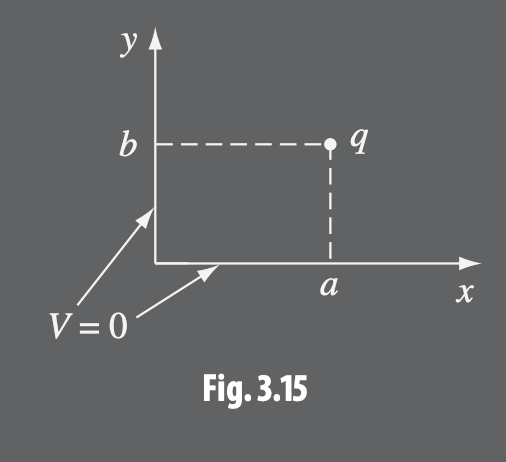
\includegraphics[width=\linewidth]{hw3_15.png}
        \caption{From Griffiths}
        \label{fig:3.15}
    \end{minipage} \hfill
    \begin{minipage}{0.45\linewidth}
        \centering
        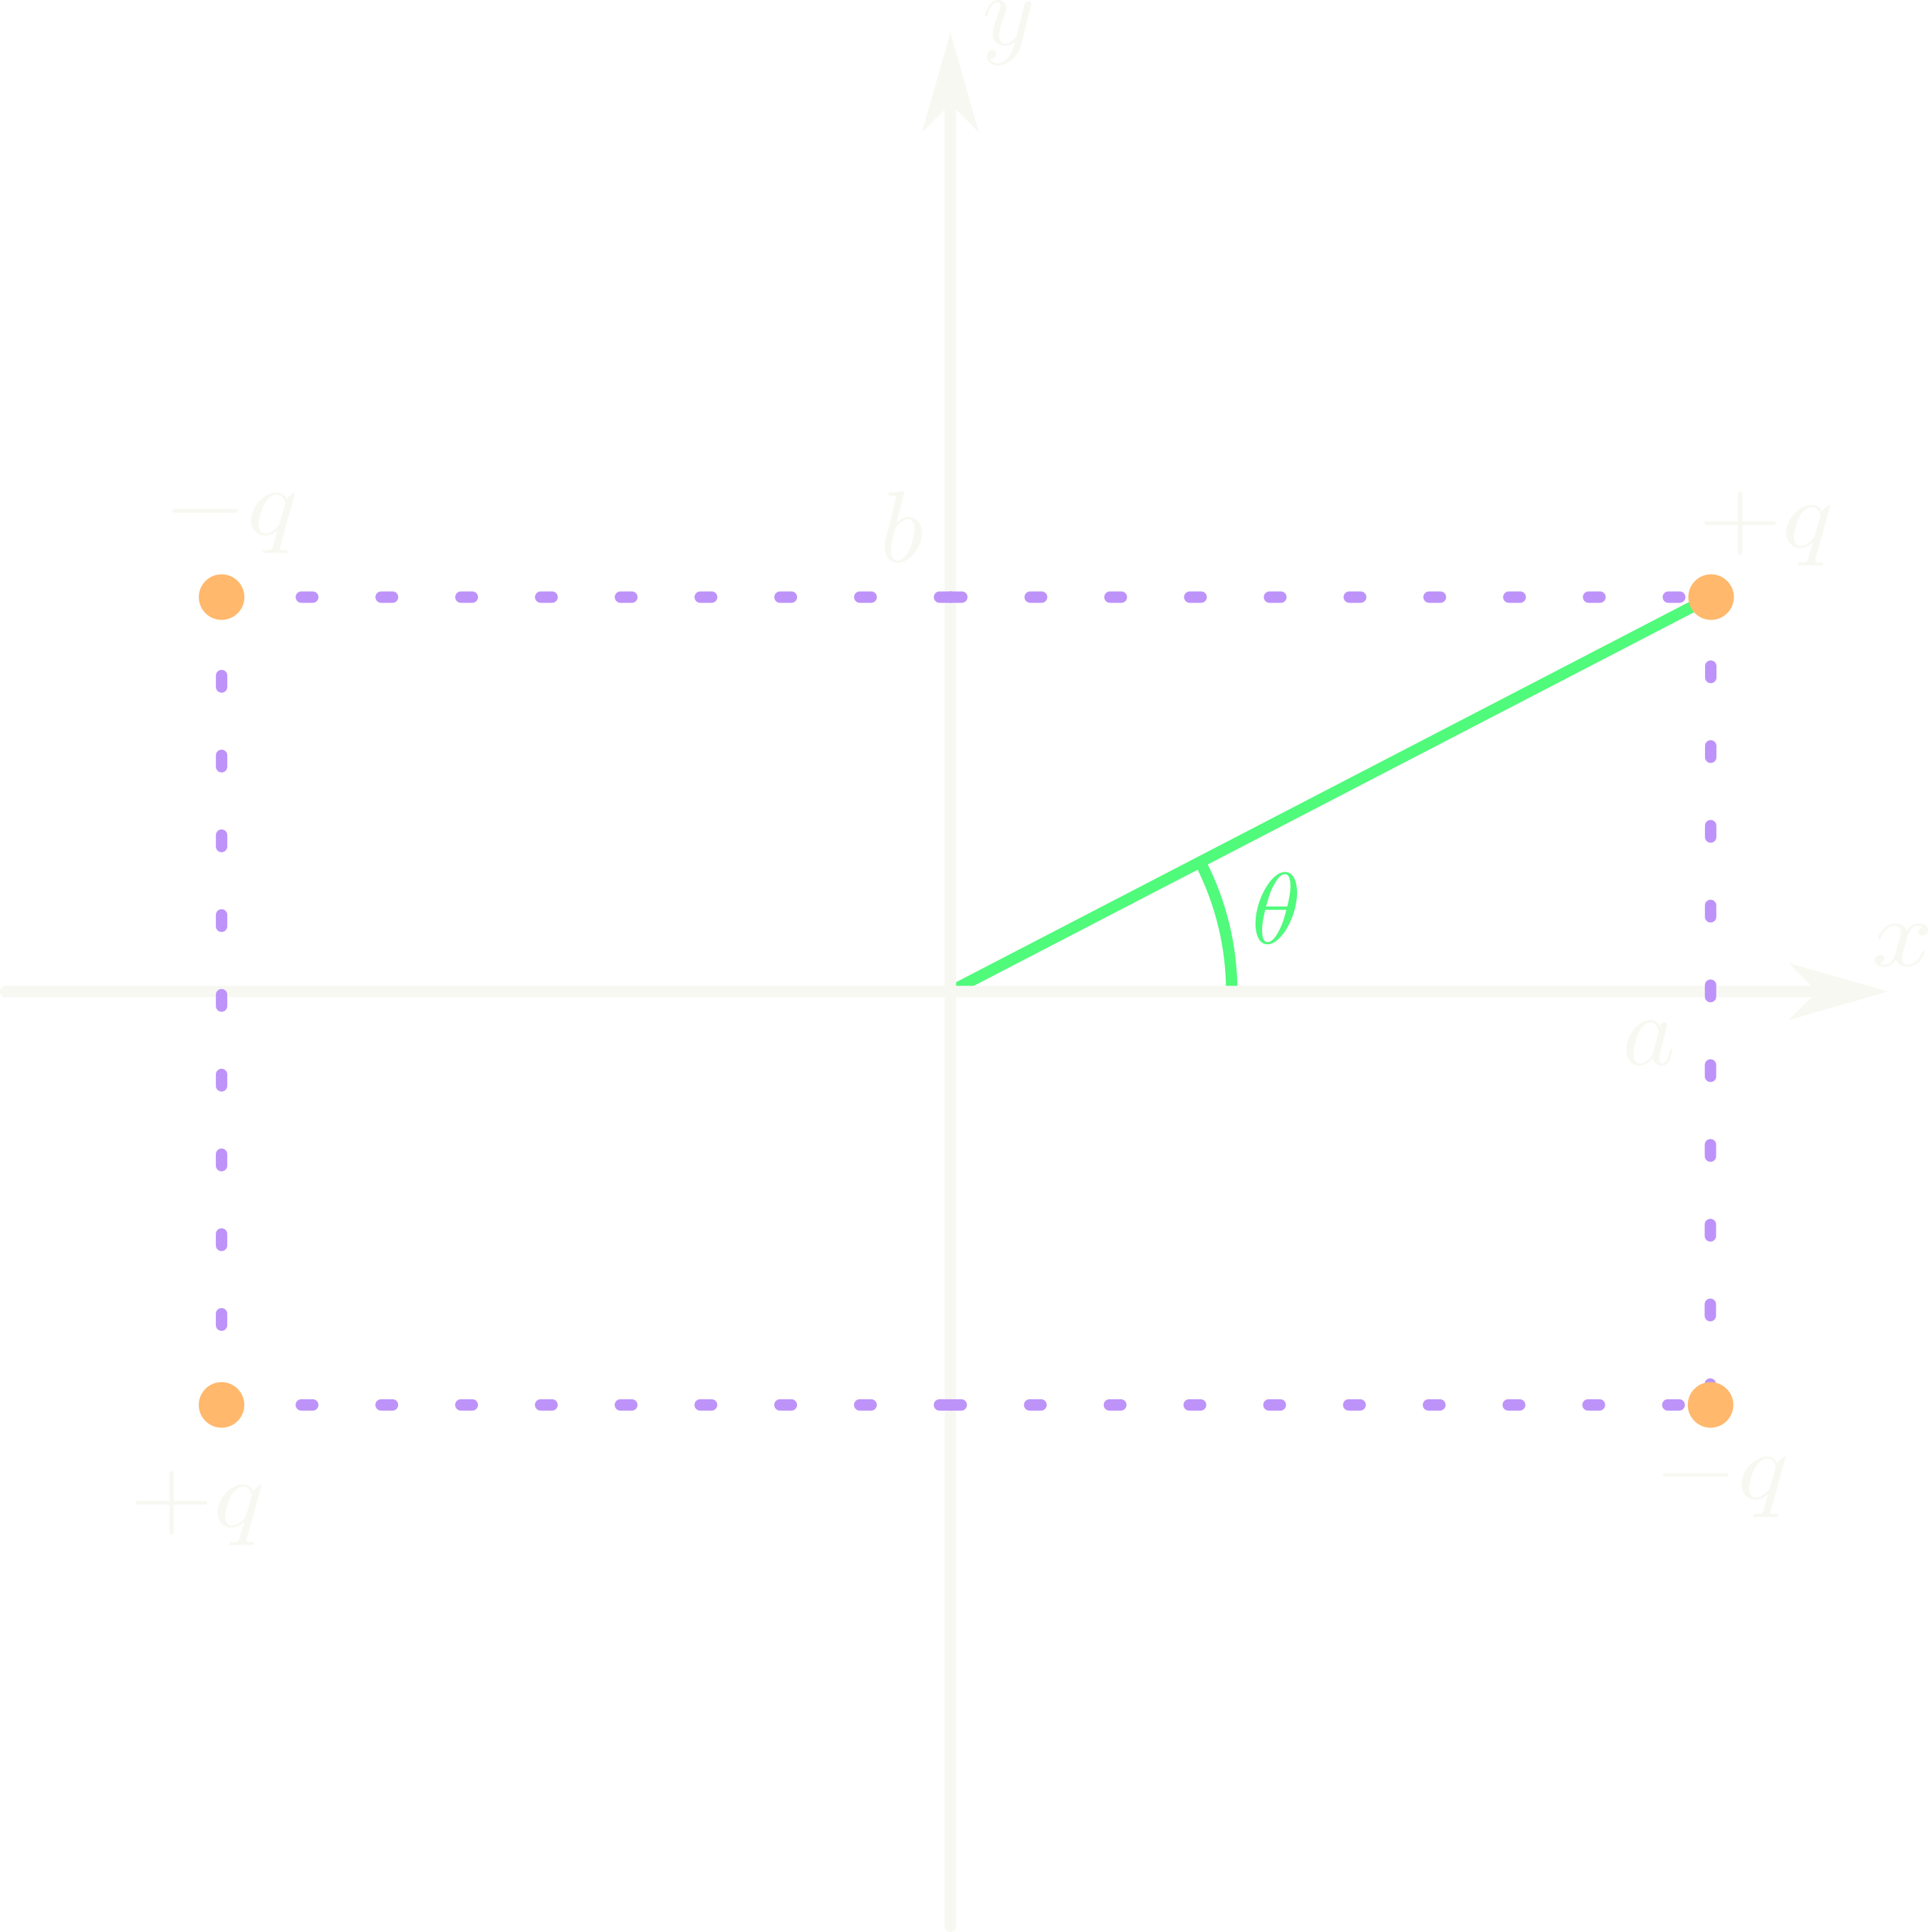
\includegraphics[width=\linewidth]{fig3_15b.png}
        \caption{Three image charges}
        \label{fig:3.15b}
    \end{minipage}
\end{figure*}
To set up the problem so we can have a potential of zero at the planes, we can place image charges $-q$ at
$(a, -b)$ and $(-a, b)$, and place an image charge $+q$ at $(-a, -b)$ to balance the potentials at the axes.

The potential in the region $x > 0, y > 0$ is:
\begin{align*}
    V = \ke q 
        &\left[ \frac{1}{\sqrt{(x - a)^2 + (y - b)^2 + z^2}} + \frac{1}{\sqrt{(x + a)^2 + (y + b)^2 + z^2}} \right. \\
        &\left. - \frac{1}{\sqrt{(x + a)^2 + (y - b)^2 + z^2}} - \frac{1}{\sqrt{(x - a)^2 + (y + b)^2 + z^2}}\right]
\end{align*}
The force on $q$ is (using Fig. \ref{fig:3.15b}):
\begin{align*}
    \vb F = \ke q^2
        &\left[ -\frac{1}{(2a)^2} \vu x - \frac{1}{(2b)^2} \vu y \right. \\
        &\left. + \frac{1}{(2\sqrt{a^2 + b^2})^2} (\cos \theta \vu x + \sin \theta \vu y) \right]
\end{align*}
where
\begin{align*}
    \cos \theta = \frac{a}{\sqrt{a^2 + b^2}} \qquad \sin \theta = \frac{b}{\sqrt{a^2 + b^2}}
\end{align*}
So 
\begin{align*}
    \vb F = \ke \frac{q^2}{4} \left[ -\frac{1}{a^2} \vu x - \frac{1}{b^2} \vu y + (\frac{a}{(a^2 + b^2)^{3/2}} \vu x + \frac{b}{(a^2 + b^2)^{3/2}} \vu y) \right] \\
    \boxed{\vb F = \frac{q^2}{16\pi \epsilon_0} \qt[
        \qt(\frac{a}{(a^2 + b^2)^{3/2}} - \frac{1}{a^2}) \vu x + \qt(\frac{b}{(a^2 + b^2)^{3/2}} - \frac{1}{b^2}) \vu y
    ]}
\end{align*}

\newpage
The work done to bring $q$ from infinity to the origin: 

Integrating the opposing force from $\infty \to (a,b)$ 
\begin{align*}
    W &= -\int_\infty^{(a, b)} \vb F \cdot \dd\ell \\
    &= - \qt[\int_{(\infty, \infty)}^{(a, \infty)} \vb F \cdot \dd \ell_a + \int_{(a, \infty)}^{(a, b)} \vb F \cdot \dd \ell_b]
\end{align*}
where
\begin{align*}
    \dd \ell_a &= \dd x \vu x + (0) \vu y = \dd x \vu x, \quad \dd \ell_b = (0) \vu x + \dd y \vu y = \dd y \vu y \\
    \implies \int_{\infty, \infty}^{(a,\infty)}\vb F \cdot \dd \ell_a &= \frac{q^2}{16 \pi \epsilon_0} \int_\infty^a \qt[
        \qt(\frac{x}{(x^2 + b^2)^{3/2}} - \frac{1}{x^2}) \dd x 
    ] \eval_{b = \infty} \\
    &= \frac{q^2}{16 \pi \epsilon_0} \int_\infty^a \qt[
        -\frac{1}{x^2} \dd x
    ] \\
    \qand \vb F \cdot \dd \ell_b &= \frac{q^2}{16 \pi \epsilon_0} \int_\infty^b \qt[
        \qt(\frac{y}{(a^2 + y^2)^{3/2}} - \frac{1}{y^2}) \dd y
    ]
\end{align*}
So the work done is
\begin{align*}
    W &= -\frac{q^2}{16\pi \epsilon_0} \qt[ \int_\infty^a 
        \qt(- \frac{1}{a^2}) \dd x
        + \int_\infty^b \qt(\frac{b}{(a^2 + b^2)^{3/2}} - \frac{1}{b^2}) \dd y
    ]
\end{align*}
Evaluating the two integrals using 
\begin{align*}
    &\int -\frac{1}{x^2} \dd x = \frac{1}{x} \\
    &\int \frac{y}{(a^2 + y^2)^{3/2}} \dd y = -\frac{1}{\sqrt{a^2 + y^2}}
\end{align*}
gives the work done is
\begin{align*}
    W &= -\frac{q^2}{16\pi \epsilon_0} \qt[
        \frac{1}{a} - \frac{1}{\sqrt{a^2 + b^2}}  + \frac{1}{b}
    ]
\end{align*}
or
\begin{align*}
    \boxed{
        W = \frac{q^2}{16\pi \epsilon_0} \qt[
            \frac{1}{\sqrt{a^2 + b^2}} - \frac{1}{a} - \frac{1}{b}
        ]
    }
\end{align*}

\newpage
We can solve the problem with the method of images, as long as the angle $\phi$ divides 180$^\circ$ into an integer,
e.g., $\phi = 180, 90, 60, 45, 36, 30, 20, 18, 15, 12, 10, 9, 6, 5, 4, 3, 2, 1, 0.5, \dots$

We would place a `mirror' at each $\phi$ division and place an image charge $-q$ that mirrors the point charge $q$ and repeat
the process with the next image charge $q$ (making sure to flip charges each time) until we have a symmetric configuration of charges as shown in Fig. \ref{fig:3.15c}.
\begin{figure*} [ht]
    \centering
    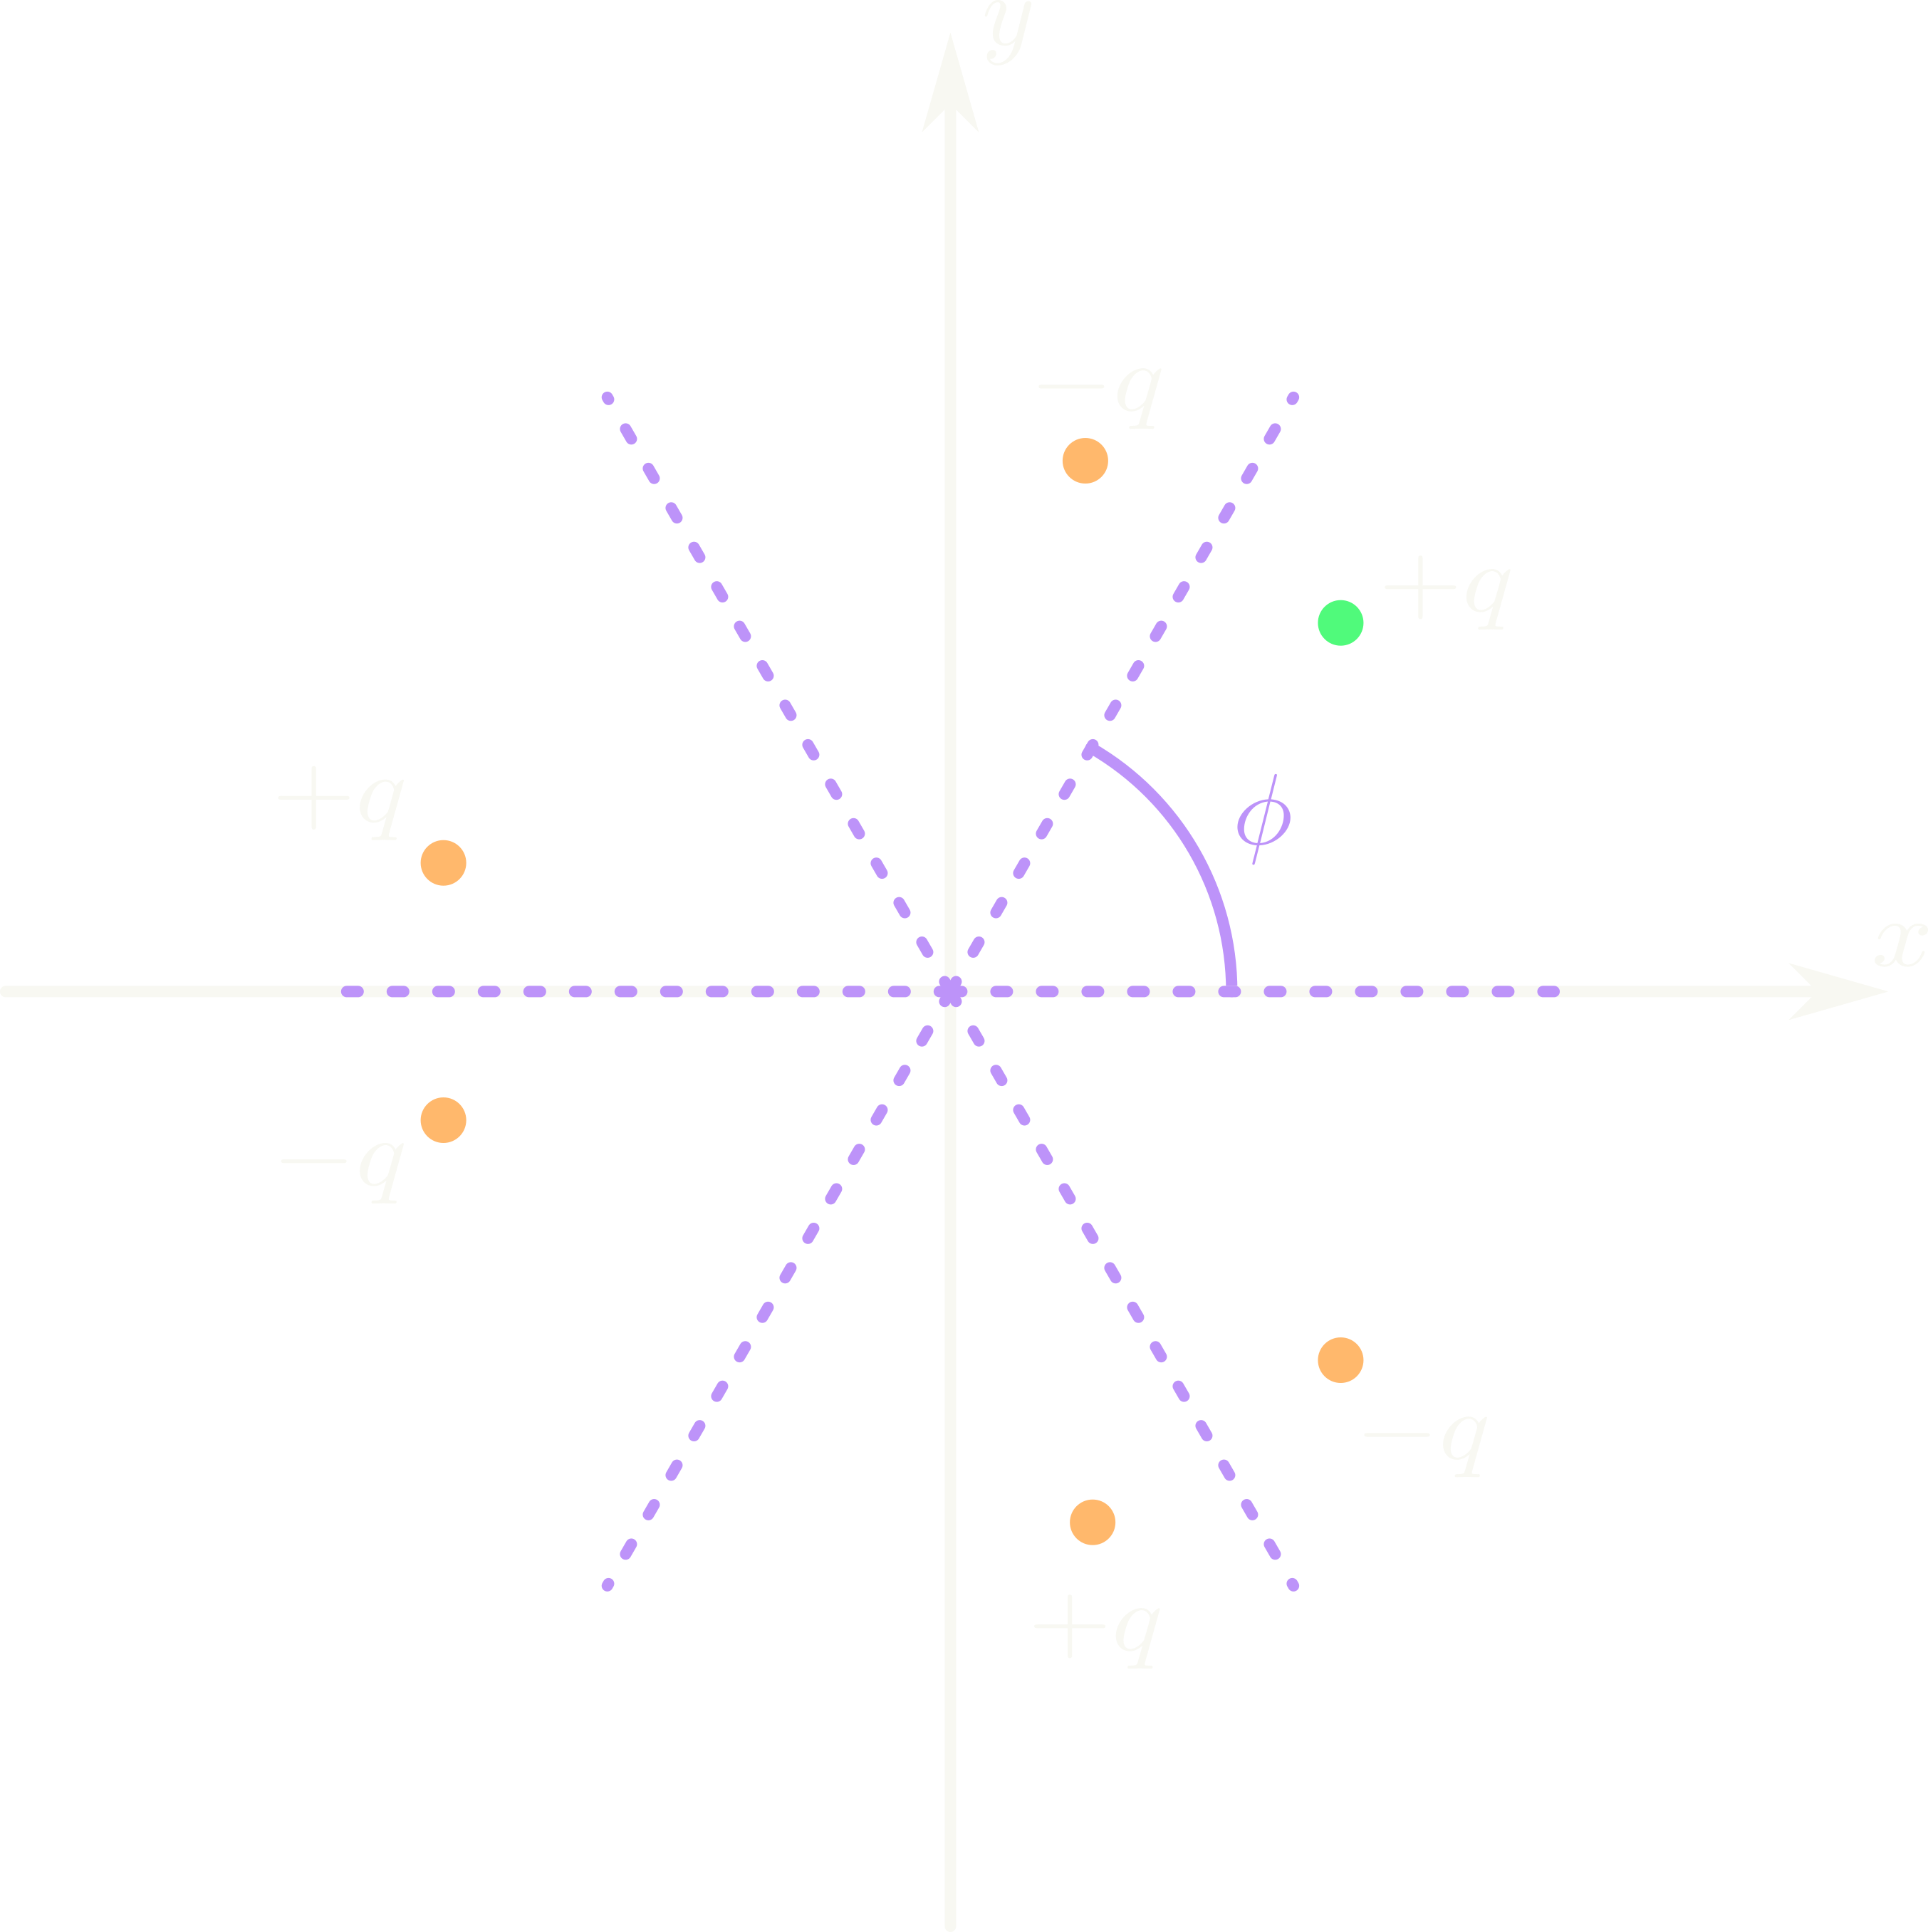
\includegraphics[width=0.5\linewidth]{hw3_15c.png}
    \caption{Method of images for $\phi = 60^\circ$}
    \label{fig:3.15c}
\end{figure*}
\end{document}